\chapter{Postproduktion}

In diesem Kapitel wird der Teil der Postproduktion beschrieben. Im Zusammenhang mit diesem Projekt ist dies das Zusammenführen von Filmmaterial und gerendertem Material im Schnitt, sowie das Nachbearbeiten dieser.

\section{Schnitt}


es stand nur schon geschnittenes footage zur verfügung
hinweis auf fernsehbeitrag des wdr (?)
daher teilweise sehr schnelle schnitte, und wenig zeit zum lesen der textinformationen

\includegraphics[width=\textwidth]{gfx/post/resolve2.jpg}

\section{Bauchbinden}

texterstellung in blender mit animation nodes

erstellung der blur kästen in resolve

\includegraphics[width=\textwidth]{gfx/post/resolve3.jpg}

\includegraphics[width=\textwidth]{gfx/post/call-out.jpg}
\includegraphics[width=\textwidth]{gfx/post/call-out2.jpg}


\section{Einfügen zusätzlicher Elemente}

iPad und Rettungsfloß wurden eingefügt mit tracking
ipad wurde auch stabilisiert

bei radiowellen war z.b. wichtig, dass der farbraum filmic erst angewendet wird, nachdem die wellen auf das flugzeug gelegt wurden. ansonsten ausbrennen oder nicht ausnutzen des farbraumes

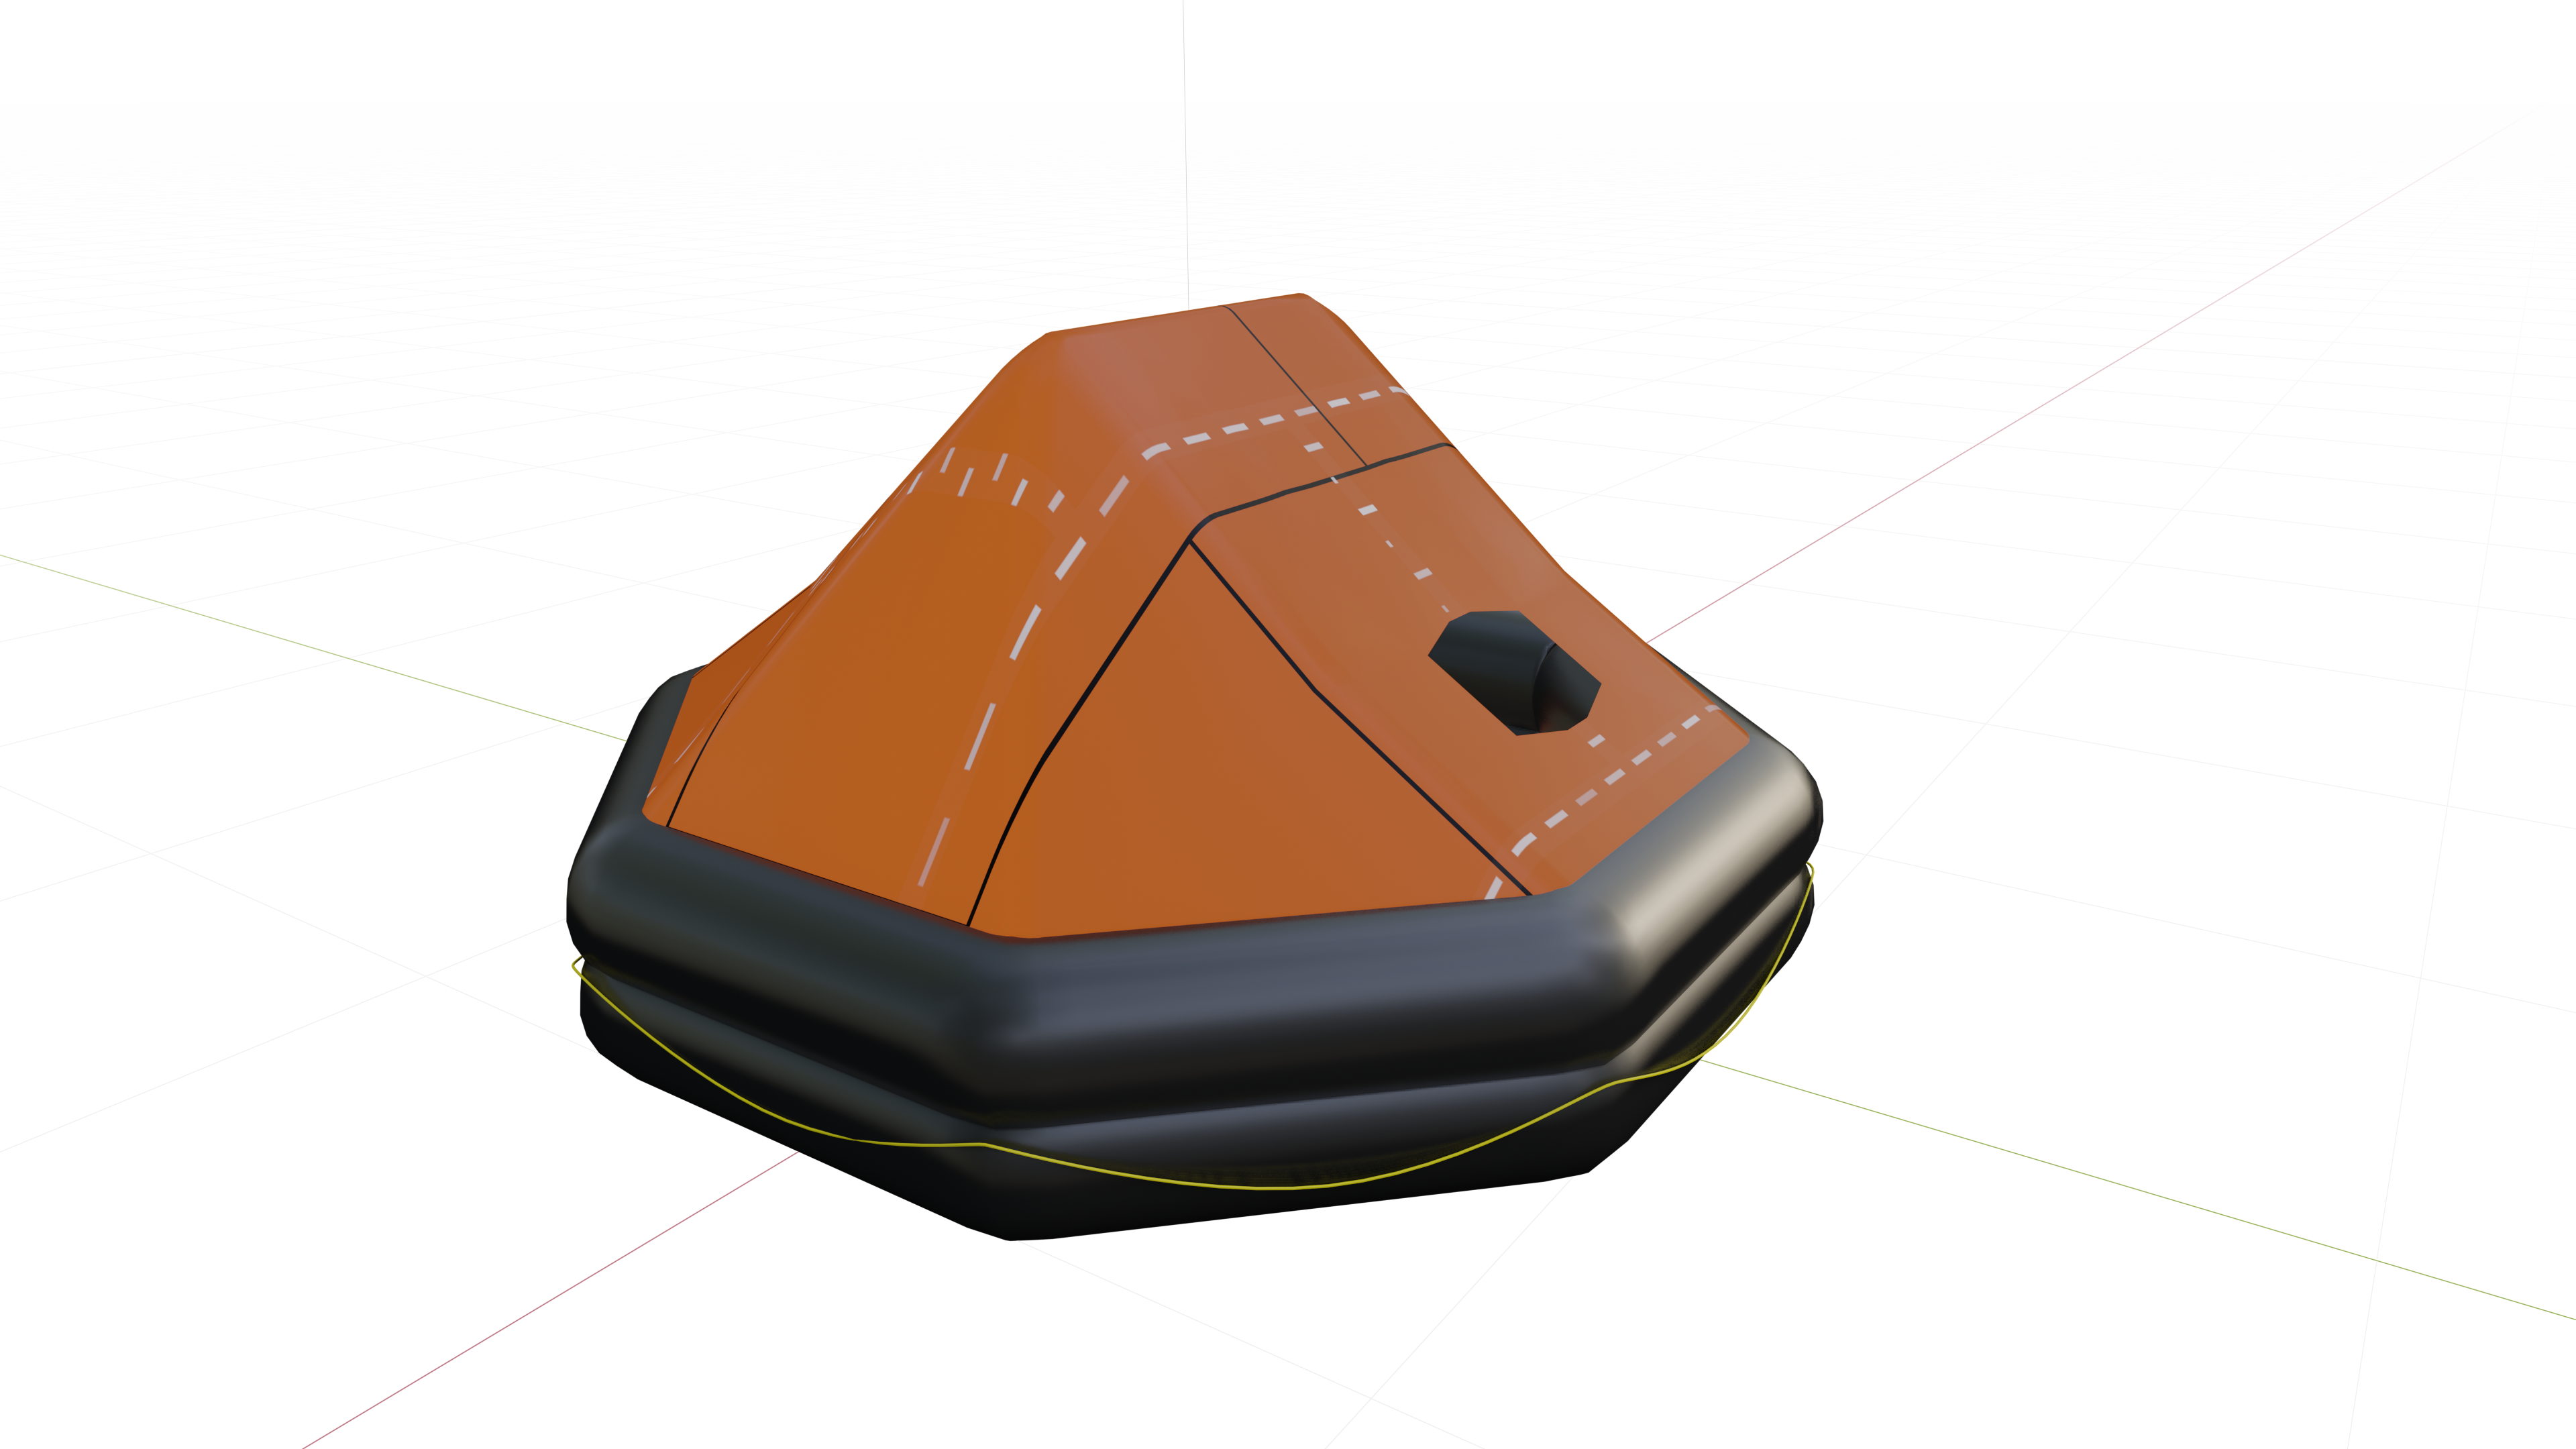
\includegraphics[width=\textwidth]{gfx/prod/boat/liferaft1.jpg}
\includegraphics[width=\textwidth]{gfx/post/resolve7.jpg}
\includegraphics[width=\textwidth]{gfx/post/resolve8.jpg}
\includegraphics[width=\textwidth]{gfx/post/resolve9.jpg}
\includegraphics[width=\textwidth]{gfx/post/resolve10.jpg}


\section{Colorgrading}

Anpassen über weißpunkt
Viel Potenzial übrig gewesen, da in openExr gerendert wurde.
dies war der zweite vorteil von exr dateien gegenüber einem klassischen dateiformat, wie bspw. jpg

davor aber noch anwenden von ocio color space wichtig, da open exr immer linear ohne farbraum ist
--> hinweis auf resolve3.jpg


\includegraphics[width=\textwidth]{gfx/post/resolve7.jpg}

\section{Audio}

musik wurde thbd ocean entschieden
passend geschnitten. eckpunkte waren hierbei der Anfang des Filmes, das Ende des Filmes.
daher wurde zuerst der titel in der mitte zerschnitten
der schnitt wurde anschließend so gewählt, dass er an einer passenden stelle ist
konkret heißt das, dass der schnitt möglichst unaufällig bei 0:56 der schnitt gesetzt wurde
ziel war damit, dass bei dem stärkeren visuellen wechsel von der seitenansicht des sichtkegels in die draufsicht die musik sich ändert
motor sample wurde kopiert und denn mehrfach nacheinander abgespielt. außerdem wurde der audio-ausschnitt manchmal gespiegelt, sodass es schwieriger zu erkennen ist, dass es sich wiederholt
Dass der Motorsound und die Musik dieselbe tonhöhe haben, war ein glücklicher zufall
WIndgeräusche

\includegraphics[width=\textwidth]{gfx/post/resolve1.jpg}
\includegraphics[width=\textwidth]{gfx/post/sample.jpg}